\section{Businesses}
	\subsection{Registration}
	If you want to create a business account for \textit{Soldino} 
	visit the homepage and make sure that the slider in set on "Business".\\
	\begin{figure}[H]
		
\includegraphics[width=5cm]{res/images/user_business.png}
		\centering
		\caption{Select "Business" from the slider}
	\end{figure}	
	\noindent Then, insert your business's data in the form. After you have completed 
	all the	fields with your informations press the "Sign up" button. If an 
	entry is not valid (i.e. the email address does not contain a valid 
	domain) the system will let you know and you have to correct that field 
	to continue. If all the informations are correct a pop up window will open 
	asking you to allow \textit{Soldino} to access your information.\\
	\begin{figure}[H]
		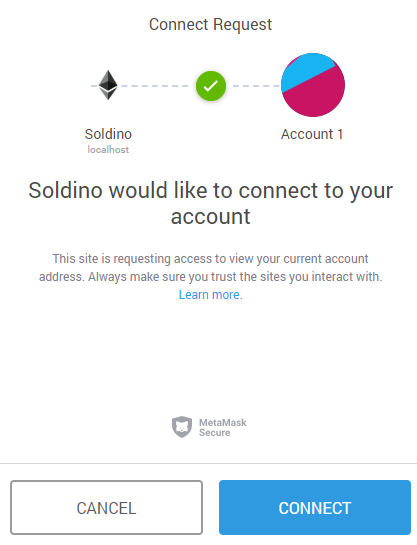
\includegraphics[width=7cm]{res/images/metamask_connect.png}
		\centering
		\caption{Connecting MetaMask to \textit{Soldino}}
	\end{figure}
	\noindent \noindent Press "Connect" and you will be redirected to a page 
	congratulating you for your registration on the platform.
	for your registration on the platform.
	\begin{figure}[H]
		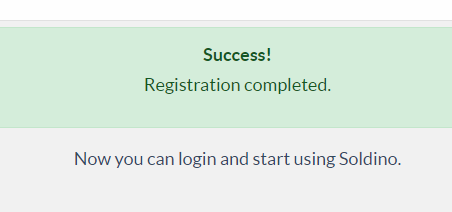
\includegraphics[width=7cm]{res/images/registration_complete.png}
		\centering
		\caption{Registration completed message}
	\end{figure}
	\subsubsection{Business is already registered}
	If your address is already registered in the platform you will see an
	error page telling you that you cannot create a new account.
	\subsection{Login}
	If you already have a personal account press the "login" button on the 
	top right of the homepage, you will automatically log in your account 
	(there is no need for a username or password, all is done via MetaMask). 
	\\To be able to log in you have to be logged in your MetaMask account.
	\subsection{Logout}
	To log out of \textit{Soldino} you just have to log out of 
	your MetaMask. To do this you have to press MetaMask's icon on the top 
	right of the browser, press your account's icon and then press "Log out"
	on the top right.
	\begin{figure}[H]
		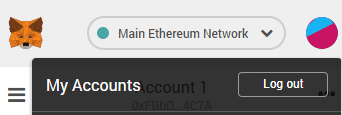
\includegraphics[width=7cm]{res/images/logout_metamask.png}
		\centering
		\caption{Registration completed message}
	\end{figure}
	\subsection{Buying}
	\subsubsection{Searching}
	You can search for products by name using the search bar that can be found 
	right at the top of the page. After you start typing you will see all 
	results that match tour search. If no matching products are found you will 
	a message showing you that.
	\subsubsection{Cart}
	You can add products in your cart, after selecting the quantity you need, 
	by pressing the "Add to cart" button under it. The number on the cart shows
	you how many different products are in it.\\
	\begin{figure}[H]
		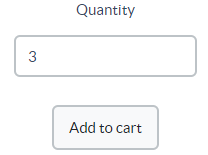
\includegraphics[width=7cm]{res/images/add_to_cart.png}
		\centering
		\caption{Adding a product to your cart}
	\end{figure}
	\noindent You can access your cart by pressing the shopping cart icon on 
	the bar at the top of the page.
	\begin{figure}[H]
		
\includegraphics[width=3cm]{res/images/cart_icon.png}
		\centering
		\caption{Icon to access your cart}
	\end{figure}
	\noindent Here you will find every item you have previously selected with 
	their quantity and above them you will see the total for your order.
	If you need to modify the quantity press the "+" or "-" buttons. \\
	\begin{figure}[H]
		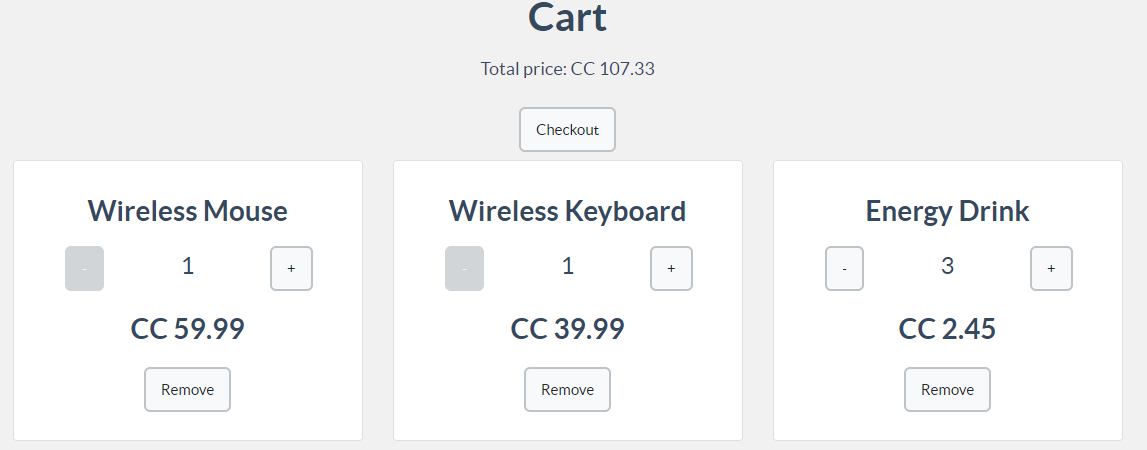
\includegraphics[width=15cm]{res/images/cart_example.png}
		\centering
		\caption{Example of content of the cart}
	\end{figure}
	\noindent When you want to proceed with the order press the "Checkout" button, 
	you will be redirected to the checkout page.
	\subsubsection{Checkout}
	In the checkout page you will be able to choose where your products will be 
	delivered to by using the radio buttons: you can either select the address you 
	gave during registration or enter a new one.\\
	\begin{figure}[H]
		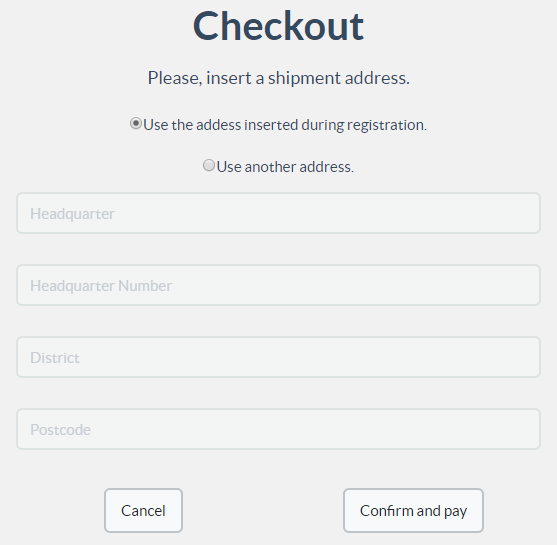
\includegraphics[width=10cm]{res/images/checkout.png}
		\centering
		\caption{Example of checkout page}
	\end{figure}
	\noindent Press the "Confirm and pay" button to proceed. In a new 
	pop up window MetaMask will ask you to confirm the transaction. The price 
	shown here will be a little higher because it includes the gas fee. \\
	Otherwise press "Cancel" to return to your cart.
	\subsubsection{Past orders}
	You can visit a the page containing all past orders by pressing the "Orders" 
	button in the bar at the top of the page.\\
	%PLACEHOLDER screen pulsante?
	Here you will find a chronological list of every purchase that you made with 
	\textit{Soldino}. Each order tells when it was made, who was the seller, 
	what were the items bought, how much you paid.
	\begin{figure}[H]
		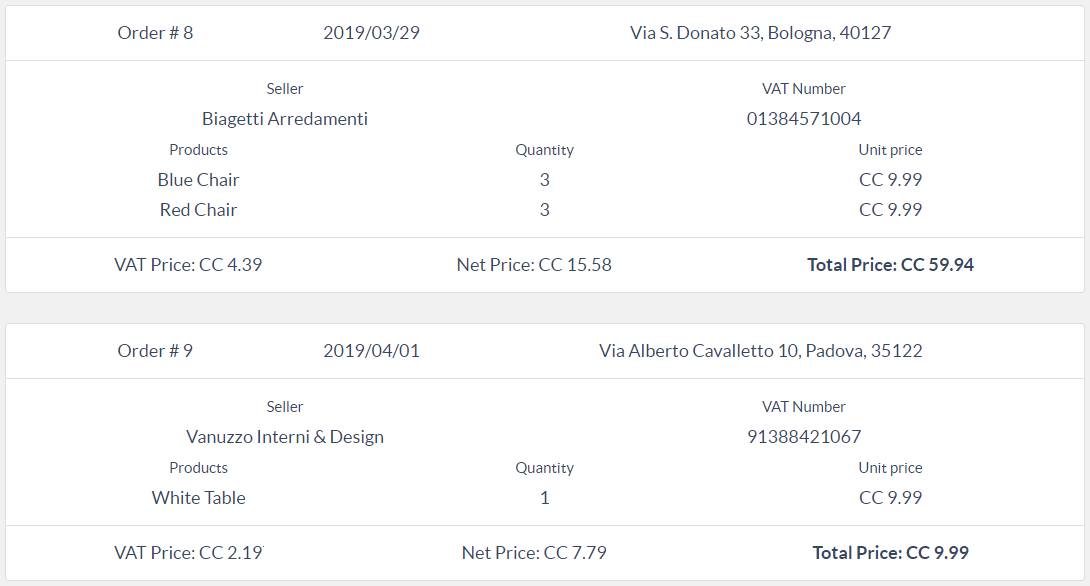
\includegraphics[width=15cm]{res/images/past_orders.png}
		\centering
		\caption{Example of past orders}
	\end{figure}

	\subsection{Selling}
	If you want to manage the products you are selling on \textit{Soldino} you 
	have to press the "Products Manager" on the bar at the top of the page. 
	Here you will find every product you are currently selling.
	\begin{figure}[H]
		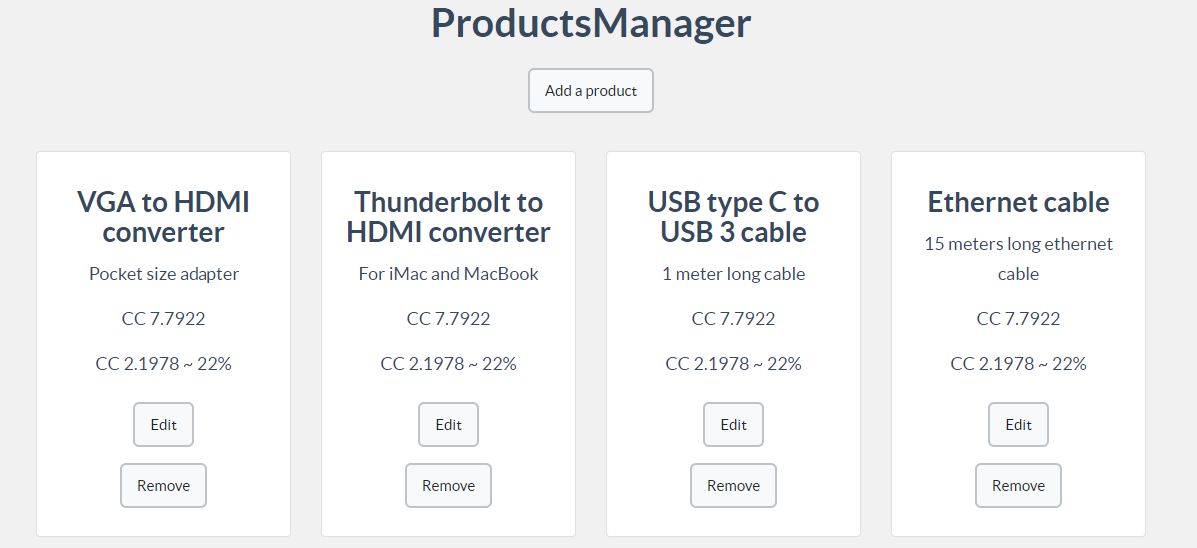
\includegraphics[width=15cm]{res/images/products_manager.png}
		\centering
		\caption{Products Manager page}
	\end{figure}
	\subsubsection{Selling a new product}
	If you want to sell a new product you have to press "Add a product", you 
	will be redirected to a page where you will have to insert all the 
	informations regarding your new product.
	\begin{figure}[H]
		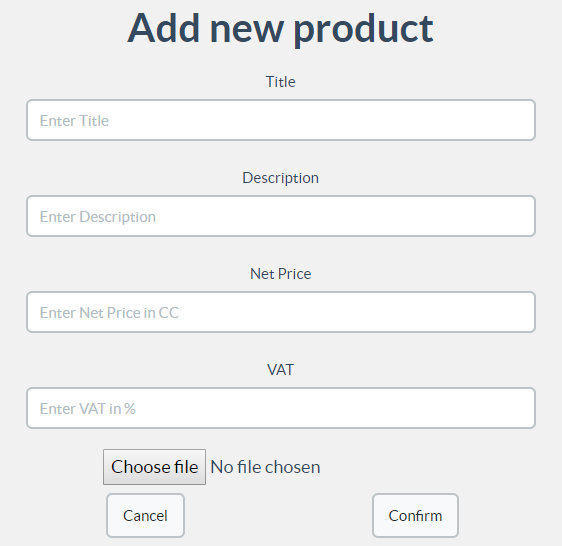
\includegraphics[width=10cm]{res/images/add_new_product.png}
		\centering
		\caption{Adding a new product}
	\end{figure}
	\noindent After you entered every information and you have selected a photo press
	"Confirm" and it will be added to the products users can buy.
	\\Press "Cancel" if you do not wish to continue.
	
	\subsubsection{Modifying a product}
	If you want to change the informations of a product you are selling press 
	the "Edit" button under them, you will be redirected to a page where you 
	will be able to change all the product's information.
	\begin{figure}[H]
		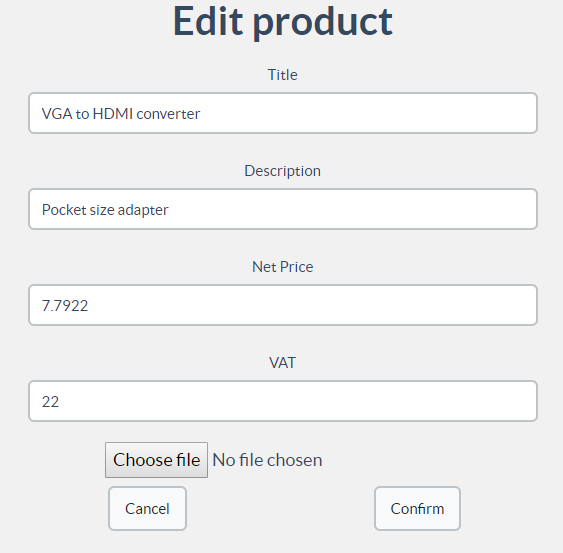
\includegraphics[width=10cm]{res/images/edit_product.png}
		\centering
		\caption{Editing a product's informations}
	\end{figure}
	\noindent After you are done with the changes press "Confirm" to save them.
	\\If you wish not to apply the changes press "Cancel".
	
	\subsubsection{Removing a product}
	If you want to remove a product you are selling from the platform press the
	"Remove" button under it.
	\\Note that removing a product will not delete orders made prior to the 
	removal. 
	
	\subsection{VAT management}
	If you are a business \textit{Soldino} will manage VAT for the products 
	you buy and sell on the platform automatically. You can access the page 
	containing all invoices by pressing the "Transaction Manager" button 
	on the bar at the top of the page.
	\begin{figure}[H]
		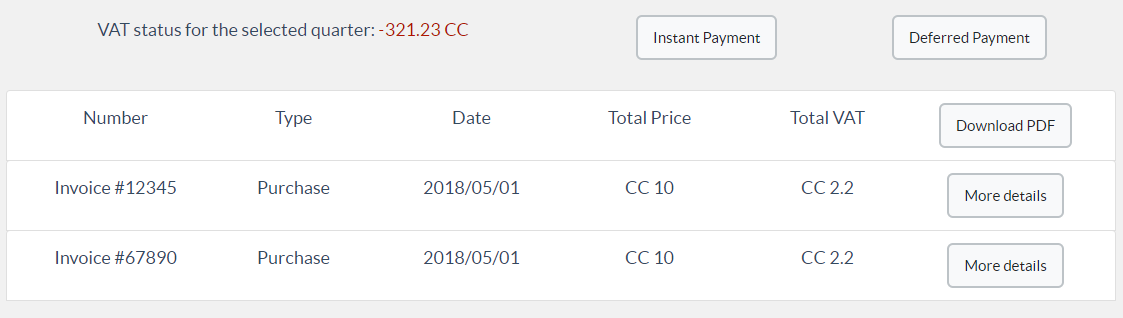
\includegraphics[width=15cm]{res/images/past_invoices.png}
		\centering
		\caption{Example of past invoices}
	\end{figure}
	\noindent Here you will also see the status of the trimester. 
	\\A red value means that you will have to pay that amount to the 
	Government.
	\begin{figure}[H]
		
\includegraphics[width=10cm]{res/images/negative_vat_status.png}
		\centering
		\caption{Example of a negative VAT status}
	\end{figure}
	\noindent While a green one means that you will soon be reimbursed for 
	that amount.
	\begin{figure}[H]
		
\includegraphics[width=10cm]{res/images/positive_vat_status.png}
		\centering
		\caption{Example of a positive VAT status}
	\end{figure}
	\noindent You can see more information about an invoice by pressing the 
	"More details" button on the right. This will open a pop up window 
	containing all the details.
	\begin{figure}[H]
		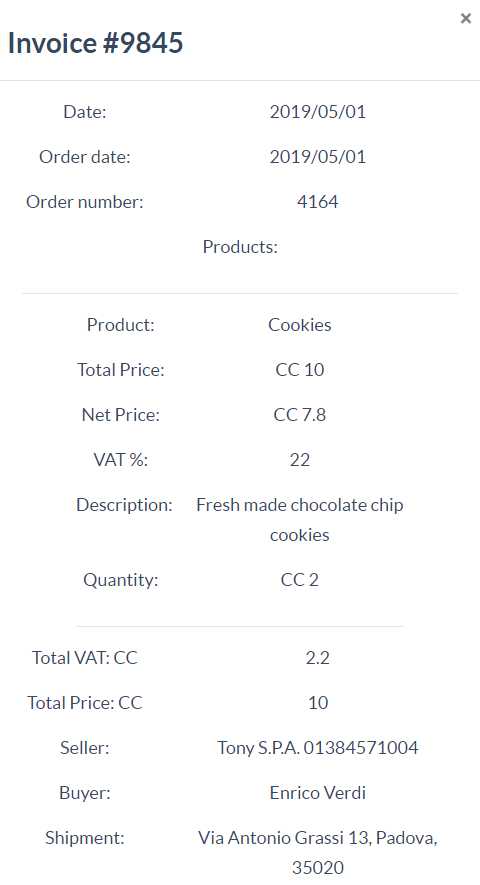
\includegraphics[width=10cm]{res/images/invoice_details.png}
		\centering
		\caption{Example of an invoice}
	\end{figure}
	\subsubsection{Paying VAT}
	If you are in debt with the government next to how much you have to pay 
	you will see two buttons.
	\begin{figure}[H]
		
\includegraphics[width=15cm]{res/images/paying_vat.png}
		\centering
		\caption{Paying off a negative Vat status}
	\end{figure}
	\paragraph{Instant payment} \mbox{}\\
	If you choose to instantly pay off what you owe by pressing "Instant 
	payment". MetaMask then will open a new window asking you allow the 
	transaction, accept to continue.
	\paragraph{Deferred payment} \mbox{}\\
	Otherwise you can defer the payment by pressing "Deferred payment" 
	\subsection{Checking past trimesters' VAT}
	You can see invoices of past trimesters by using the drop-down 
	menu at the top of the page.
	\begin{figure}[H]
		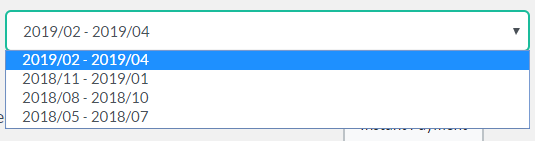
\includegraphics[width=10cm]{res/images/past_trimesters.png}
		\centering
		\caption{Past trimesters}
	\end{figure}
	\noindent From this page you will also be able to see invoices' specific 
	details or download them as PDF as explained before.